\documentclass[11pt, a4paper]{article}
\usepackage[utf8]{inputenc}
\usepackage[english]{babel}
\usepackage{amsmath}
\usepackage{amsfonts}
\usepackage{amssymb}
\usepackage{graphicx}
\usepackage{array}
\usepackage{tikz}
\usepackage{listings}
\usepackage[justification=centering]{caption}
\usetikzlibrary{arrows, automata, graphs, shapes, petri, decorations.pathmorphing}

\renewcommand{\labelenumi}{(\roman{enumi})}

\author{Niklas Rieken}
\title{Äquivalenzsatz von Kleene}


\begin{document}
\maketitle

In diesem Dokument geht es um die Äquivalenz von regulären Ausdrücken und endlichen Automaten. Stephen C. Kleene zeigte, dass es zu jedem regulären Ausdruck einen DFA(!) gibt und umgekehrt. Der Beweis damals war aufgrund des fehlenden Konzept des \textit{Nichtdeterminismus} ziemlich abgedreht (denkt mal drüber nach, wie man es anstellt aus einem Regex sofort einen DFA zu bauen). Dieses Dokument entstand auf Grundlage eines Übungsblattes aus dem Sommersemester 2016 und wurde für die Notation von Professor Rossmanith 2017 etwas überarbeitet.

\subsection*{Reguläre Ausdrücke}
Reguläre Ausdrücke sind induktiv aufgebaut und beschreiben immer eine reguläre Sprache, welche mit den FA-erkennbaren Sprachen zusammenfallen (Satz von Kleene).\par
Reguläre Ausdrücke sind wie folgt definiert:\\
Basisfälle: \( \emptyset, \varepsilon \) und \( a \) sind reguläre Ausdrücke für jedes \( a \in \Sigma \).\\
Rekursionsschritt: Sind \( r \) und \( e \) reguläre Ausdrücke, so sind auch \( (r \cdot e), (r + e) \) und \( r^\ast \) reguläre Ausdrücke.\\
Semantisch stehen die Ausdrücke \( \emptyset, \varepsilon, a \) für die Sprachen \( L(\emptyset) := \emptyset, L(\varepsilon) := \{ \varepsilon \}, L(a) := \{ a \} \) und im rekursiven Fall \( L(r \cdot e) := L(r) \cdot L(e), L(r + e) := L(r) \cup L(e), L(r^\ast) := L(r)^\ast \). Klammern und \( \cdot \) werden gerne auch weggelassen, wenn der Ausdruck auch so klar ist.\par
Gelegentlich kennen Studenten reguläre Ausdrücke bereits durch Programme wie \texttt{grep, sed, vim}, womit sich Textdateien u.a. durchsuchen lassen mithilfe von POSIX-Ausdrücken. Diese sind gleichmächtig mit denen aus der Vorlesung, sollten aber nicht verwendet werden. Man möchte die Anzahl der Rekursionen auf das Minimum reduzieren, da dadurch auch die Beweise über reguläre Ausdrücke kürzer werden. Auf POSIX-Shortcuts wie \( (r?) \) für \( (r + \varepsilon) \), Umbenennungen wie \( (r|e) \) für \( (r + e) \) oder Schreibweisen wie \( [a-c] \) für \( (a + b + c) \) solltet ihr also verzichten. Die einzige Ausnahme ist hier vielleicht \( r^+ \) für \( rr^\ast \).\par
Aus den Tutoraufgaben eines alten Übungsblattes hier zwei Beispiele nun:
\begin{description}
	\item[a)] \( L_1 = \{ w \in \{ a, b, c \}^\ast \mid w \text{ hat gerade Länge } \} \).\\
		\( r_1 = ((a+b+c)(a+b+c))^\ast \). Dass dieser Ausdruck die Sprache beschreibt lässt sich wie gewohnt über Induktion beweisen (zwei Richtungen für Gleichheit). Das ist aber hier nicht gefordert.
	\item[c)] \( L_3 = \{ w \in \{ a, b, c \}^+ \mid \text{erstes und letztes Symbol sind gleich} \} \).\\
		\( r_3 = a(a+b+c)^\ast a + b(a+b+c)^\ast b + c(a+b+c)^\ast c + a + b + c \). Hier werden die Spezialfälle für \( \left| w \right| = 1 \) gerne übersehen.
\end{description}
Statt \( (a+b+c) \) schreibt man gerne auch einfach \( \Sigma \). Das ist aber eigentlich nicht ganz korrekt, da wir zwischen regulären Ausdrücken und den Sprachen die sie beschreiben unterscheiden. (\( r \) vs. \( L(r) \)). Streng genommen sind demnach auch die Zeichen \( \emptyset, \varepsilon, a \), wie oben in der Definition der regulären Ausdrücke, verschieden von den der Sprache \( \emptyset \), dem leeren Wort \( \varepsilon \) und dem Symbol \( a \in \Sigma \). Wenn man also wie in Aufgabe a) z.B. \( (\Sigma\Sigma)^\ast \) schreiben möchte, sollte man sich zumindest vorher \( \Sigma \) als regulären Ausdruck \( \Sigma := (a+b+c) \) definieren.


\subsection*{Von Automaten zu regulären Ausdrücken (Floyd-Warshall-Algorithmus)}
Das Verfahren was hier beschrieben wird ist etwas schreibaufwändig (im Vergleich zum State-Elimination-Algorithmus von Prof. Thomas), es ist aber das von Prof. Grohe präferierte Verfahren und wird in ähnlicher Form auch bei Prof. Rossmanith durchgeführt, deshalb müssen wir da jetzt durch. Die Idee ist eigentlich sogar recht einfach: Wir wollen vom Startzustand \( q_1 \) alle möglichen Pfade (d.h. über alle möglichen Zustände) zu akzeptierenden Zuständen finden (hier im Beispiel aus Abbildung~\ref{fig:dfa} nur \( q_1 \)). Allgemein suchen wir den regulären Ausdruck
\[
	r = \sum_{q_j \in F} r_{1j}^n = r_{1j_1}^n + \ldots + r_{1j_\ell}^n
\]
wobei \( q_{j_1}, \ldots, q_{j_\ell} \in F \). Die Notation funktioniert folgendermaßen: Ein regulärer Ausdruck \( r_{ij}^k \) mit \( 0 \leq k \leq n := \left| Q \right| \) und \( q_i, q_j \in Q \) beschreibt die Wörter mit denen man von \( q_i \) nach \( q_j \) kommt und dabei nur die Zustände \( q_1, \ldots, q_k \) benutzt. Dies lässt sich rekursiv nun runterbrechen durch folgende Basisfälle:
\[
	r_{ij}^0 = \left\lbrace 
		\begin{array}{*3{>{\displaystyle}l}p{5cm}}
			\ &\sum_{a \in \Sigma: \delta(q_i, a) = q_j} a, & i \neq j\\
			\varepsilon + &\sum_{a \in \Sigma: \delta(q_i, a) = q_j} a, & i = j.
		\end{array}
	\right.	
\]
Anschaulich meint das: Alle Symbole die im Transitionsgraphen auf der Kante von \( q_i \) nach \( q_j \) stehen durch \( + \) verbunden. Sollte keine Transition existieren, dann ist der reguläre Ausdruck entsprechend \( \emptyset \) für \( q_i \neq q_j \) und \( \varepsilon \) für \( q_i = q_j \).\\
Der Rekursionsschritt funktioniert nun folgendermaßen: Für ein \( k > 0 \) ''eliminieren`` wir den Zustand \( q_k \) durch folgende Rekursion:
\[
	r_{i,j}^k = r_{ij}^{k-1} + r_{ik}^{k-1} r_{kk}^{k-1\ast} r_{kj}^{k-1}.
\]
Auch dies einmal in einfache Worte gefasst: Um von \( q_i \) nach \( q_j \) zu kommen, ausschließlich mit den Zuständen \( q_1, \ldots, q_k \) können wir entweder (links vom +) von \( q_i \) nach \( q_j \) gehen ohne den Zustand \( q_k \) zu besuchen oder (rechts vom +) von \( q_i \) nach \( q_k \) gehen, Pfade von \( q_k \) nach \( q_k \) benutzen und schließlich von \( q_k \) nach \( q_j \) gehen, wobei wir in jedem Zwischenschritt nur noch Transitionen über Zustände \( q_1, \ldots, q_{k-1} \) benutzen.\\
Diesen rekursiven Schritt habe ich nochmal in Abbildung~\ref{fig:fwa} veranschaulicht.
\begin{figure}
	\centering
	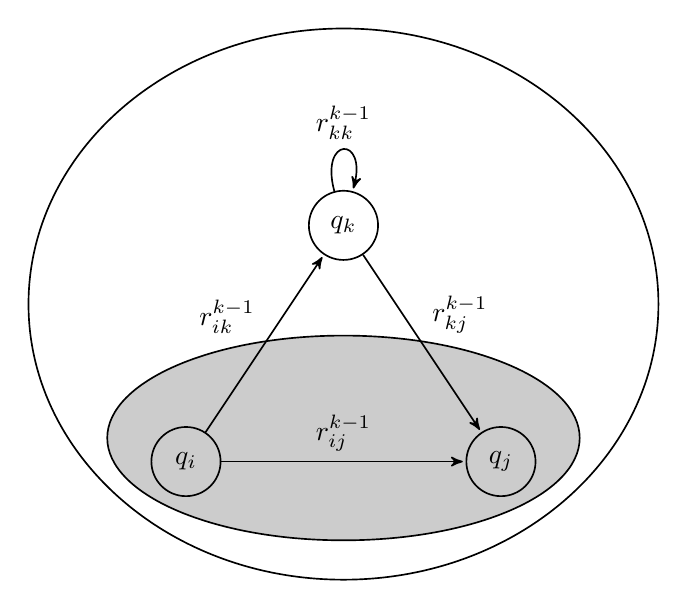
\begin{tikzpicture}[->, >=stealth', shorten >=1pt, auto, semithick]
		\draw[black, fill=black!20] (2, .3) circle[x radius=3, y radius= 1.3];
		\draw[black] (2, 2) circle[x radius=4, y radius=3.5];
		
		\node[state] (i) at (0, 0) {$q_i$};
		\node[state] (j) at (4, 0) {$q_j$};
		\node[state] (k) at (2, 3) {$q_k$};
		
		\path (i) edge node {$r_{ij}^{k-1}$} (j)
			(i) edge node {$r_{ik}^{k-1}$} (k)
			(k) edge[loop above] node {$r_{kk}^{k-1}$} (k) % curly loop
			(k) edge node {$r_{kj}^{k-1}$} (j);
	\end{tikzpicture}
	\caption{Rekursionsschritt um einen Zustand rauszuwerfen. Die grau getönte Fläche besteht nur aus den Zuständen \( q_1, \ldots, q_{k-1} \). Die größere Fläche enthält zusätzlich den Zustand \( q_k \), sonst keinen weiteren. Wichtig: Die Kanten in diesem Graphen sind keine Transitionen, sondern sind mit einem regulären Ausdruck beschriftet, der die Sprache zwischen den Knoten beschreibt mit Zuständen aus dem Index!}
	\label{fig:fwa}
\end{figure}
Falls das Verfahren jemanden bekannt vorkommt, könnte derjenige damit richtig liegen. Es handelt sich bei dem Algorithmus um eine Version des \textit{Floyd-Warshall-Algorithmus}, der in ''Datenstrukturen und Algorithmen`` in der Regel auch vorgestellt wird um günstigste Pfade in gewichteten Graphen zu finden.\par
Die Aufgabe selbst gehe ich jetzt nicht komplett durch, aber ein paar Rekursionsschritte sollten genügen um die Idee zu verstehen.
\begin{figure}[h]
	\centering
	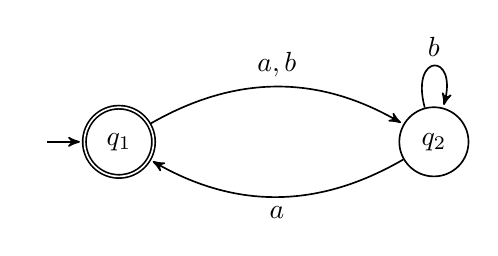
\begin{tikzpicture}[->, >=stealth', shorten >=1pt, auto, semithick]
		\node[state, initial, accepting, initial text=] (q1) at (0, 0) {$q_1$};
		\node[state] (q2) at (4, 0) {$q_2$};
		
		\path (q1) edge[bend left] node {$a, b$} (q2)
        (q2) edge[loop above] node {$b$} (q2)
		(q2) edge[bend left] node {$a$} (q1);   
	\end{tikzpicture}
	\caption{Ein DFA}
	\label{fig:dfa}
\end{figure}
Wir suchen also einen regulären Ausdruck, der die Worte beschreibt mit denen man von \( q_1 \) nach \( q_1 \) kommt mit allen Zuständen, also den Ausdruck \( r_{11}^2 \). Wir eliminieren nun \( q_2 \)
\[
	r_{11}^2 = r_{11}^1 + r_{12}^1 r_{22}^{1\ast} r_{21}^1.
\]
Noch zu berechnen sind also \( r_{11}^1, r_{12}^1, r_{22}^1, r_{21}^1 \).
\begin{align*}
	r_{11}^1 &= r_{11}^0 + r_{11}^0 r_{11}^{0\ast} r_{11}^0\\
	r_{12}^1 &= r_{12}^0 + r_{11}^0 r_{11}^{0\ast} r_{12}^0\\
	r_{22}^1 &= r_{22}^0 + r_{21}^0 r_{11}^{0\ast} r_{12}^0\\
	r_{21}^1 &= r_{21}^0 + r_{21}^0 r_{11}^{0\ast} r_{11}^0.
\end{align*}
Wir können nun für die Ausdrücke \( r_{11}^0, r_{12}^0, r_{22}^0, r_{21}^0 \) den Basisfall anwenden:
\begin{align*}
	r_{11}^0 &= \varepsilon + \emptyset \equiv \varepsilon\\
	r_{12}^0 &= a + b\\
	r_{22}^0 &= \varepsilon + b\\
	r_{21}^0 &= a.
\end{align*}
Dies können wir nun wieder rekursiv einsetzen, wir vereinfachen außerdem auch noch. In den Hausaufgaben ist dies nicht notwendig:
\begin{align*}
	r_{11}^1 &= \varepsilon + \varepsilon \varepsilon^\ast \varepsilon &&\equiv \varepsilon\\
	r_{12}^1 &= (a + b) + \varepsilon \varepsilon^\ast (a + b) &&\equiv a + b\\
	r_{22}^1 &= (\varepsilon + b) + (a \varepsilon^\ast (a + b)) &&\equiv \varepsilon + b + a(a + b)\\
	r_{21}^1 &= a + a \varepsilon^\ast \varepsilon &&\equiv a.
\end{align*}
Und weiter:
\[
	r_{11}^2 = \varepsilon + (a + b) (\varepsilon + b + a(a+b))^\ast a \equiv \varepsilon + (a + b)(b + a(a+b))^\ast a.
\]

\subsection*{Von regulären Ausdrücken zu Automaten (Thompson-Konstruktion)}
Die andere Richtung, von regulären Ausdrücken zu endlichen Automaten ist deutlich bequemer mit der \textit{Thompson-Konstruktion}. Eine Variante davon wurde in der Vorlesung vorgestellt. Durch die rekursive Definition von regulären Ausdrücken lässt sich aus einem Ausdruck auch rekursiv ein \(\varepsilon\)-NFA aufbauen:
Basisfälle: In Abbilungen~\ref{fig:empty},~\ref{fig:eps} und~\ref{fig:a}.
\begin{figure}[h]
	\begin{minipage}{.3\textwidth}
	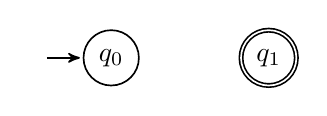
\begin{tikzpicture}[->, >=stealth', shorten >=1pt, auto, semithick, every state/.style={inner sep=0pt, minimum size=20pt}]
		\node[state, initial, initial text=]	(0) at (0, 0) {$q_0$};
		\node[state, accepting] 				(1) at (2, 0) {$q_1$};
	\end{tikzpicture}
	\caption{\( r = \emptyset \)}
	\label{fig:empty}
	\end{minipage}
	\begin{minipage}{.3\textwidth}
	\begin{tikzpicture}[->, >=stealth', shorten >=1pt, auto, semithick, every state/.style={inner sep=0pt, minimum size=20pt}]
		\node[state, initial, initial text=] (0) at (0, 0) {$q_0$};
		\node[state, accepting] (0) at (0, 0) {$q_1$};
		\path (0) edge node {$\varepsilon$} (1);
	\end{tikzpicture}
	\caption{\( r = \varepsilon \)}
	\label{fig:eps}
	\end{minipage}
	\begin{minipage}{.3\textwidth}
	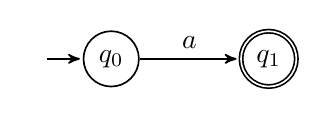
\begin{tikzpicture}[->, >=stealth', shorten >=1pt, auto, semithick, every state/.style={inner sep=0pt, minimum size=20pt}]
		\node[state, initial, initial text=] (0) at (0, 0) {$q_0$};
		\node[state, accepting] (1) at (2, 0) {$q_1$};
		\path (0) edge node {$a$} (1);
	\end{tikzpicture}
	\caption{\( r = a \)}
	\label{fig:a}
	\end{minipage}
\end{figure}
Rekursive Fälle: Seien \( \mathcal{A}_e, \mathcal{A}_{e^\prime} \) \( \varepsilon \)-NFAs für die regulären Ausdrücke \( e, e^\prime \) mit Startzuständen \( q_0, q_0^\prime \) und akzeptierenden Zuständen \( q_f, q_f^\prime \) (in dieser Variante haben wir ein paar nette Invarianten: 1. Es gibt nur einen Endzustand egal wie groß oder verschachtelt der reguläre Ausdruck ist, 2. der Startzustand hat keine eingehende Transition, 3. Der Endzustand hat keine ausgehende Transition). In den Abbildungen~\ref{fig:plus},~\ref{fig:dot} und~\ref{fig:star} ist dargestellt wie die Komposition mit \( +, \cdot \) und~\( ^\ast \) funktioniert.\\
\begin{figure}[h]
	\centering
	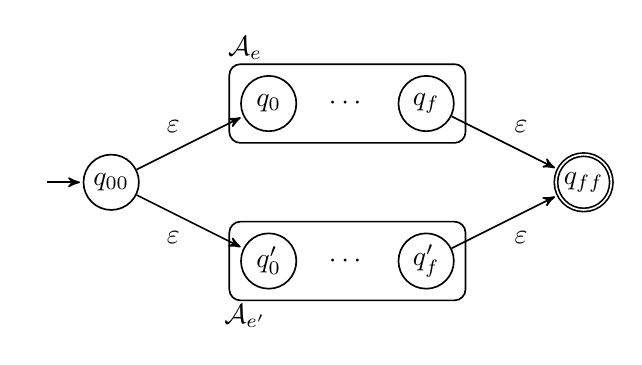
\begin{tikzpicture}[->, >=stealth', shorten >=1pt, auto, semithick, every state/.style={inner sep=0pt, minimum size=20pt}]
		\node[state, initial, initial text=] (0) at (0, 0) {$q_{00}$};
		
		\node at (1.7, 1.7) {$\mathcal{A}_e$};
		\draw[black, rounded corners] (1.5, 1.5) rectangle (4.5, .5);
		\node[state] (1) at (2, 1) {$q_0$};
		\node[state] (2) at (4, 1) {$q_f$};
		\node (d1) at (3, 1) {$\cdots$};
		
		\node at (1.7, -1.7) {$\mathcal{A}_{e^\prime}$};
		\draw[black, rounded corners] (1.5, -1.5) rectangle (4.5, -.5);
		\node[state] (3) at (2, -1) {$q_0^\prime$};
		\node[state] (4) at (4, -1) {$q_f^\prime$};
		\node (d2) at (3, -1) {$\cdots$};
		
		\node[state, accepting] (5) at (6, 0) {$q_{ff}$};
		
		\path (0) edge node {$\varepsilon$} (1)
			(0) edge node[below left] {$\varepsilon$} (3)
			(2) edge node {$\varepsilon$} (5)
			(4) edge node[below right] {$\varepsilon$} (5);	
	\end{tikzpicture}
	\caption{\( r = e + e^\prime \)}
	\label{fig:plus}
\end{figure}
\begin{figure}[h]
	\centering
	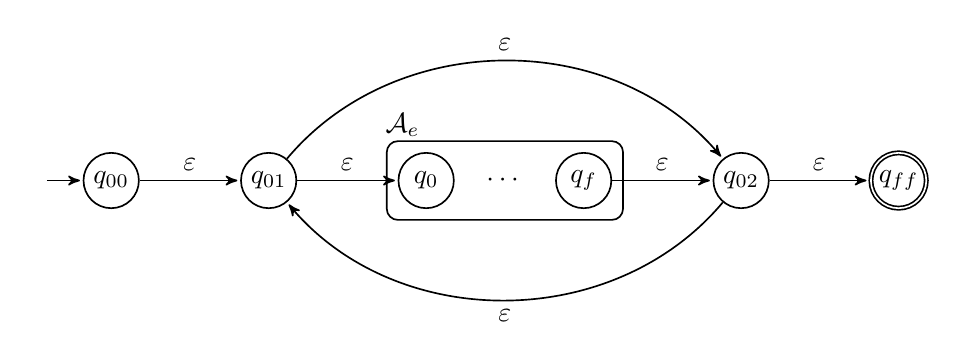
\begin{tikzpicture}[->, >=stealth', shorten >=1pt, auto, semithick, every state/.style={inner sep=0pt, minimum size=20pt}]
		\node[state, initial, initial text=] (0) at (-2, 0) {$q_{00}$};
		\node[state] (01) at (0, 0) {$q_{01}$};
		\node[state] (02) at (6, 0) {$q_{02}$};
		\node[state, accepting] (ff) at (8, 0) {$q_{ff}$};
		
		\node at (1.7, .7) {$\mathcal{A}_e$};
		\draw[black, rounded corners] (1.5, .5) rectangle (4.5, -.5);
		\node[state] (1) at (2, 0) {$q_0$};
		\node[state] (2) at (4, 0) {$q_f$};
		\node (d1) at (3, 0) {$\cdots$};
		
		\path (0) edge node {$\varepsilon$} (01)
			(01) edge node {$\varepsilon$} (1)
			(01) edge[bend left=50] node {$\varepsilon$} (02)
			(02) edge[bend left=50] node {$\varepsilon$} (01)
			(2) edge node {$\varepsilon$} (02)
			(02) edge node {$\varepsilon$} (ff);
	\end{tikzpicture}
	\caption{\( r = e^\ast \)}
	\label{fig:star}
\end{figure}
\begin{figure}[h]
	\centering
	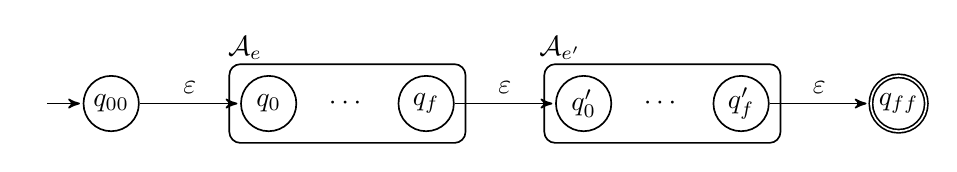
\begin{tikzpicture}[->, >=stealth', shorten >=1pt, auto, semithick, every state/.style={inner sep=0pt, minimum size=20pt}]
		\node at (1.7, .7) {$\mathcal{A}_e$};
		\draw[black, rounded corners] (1.5, .5) rectangle (4.5, -.5);
		\node[initial, initial text=, state] (0) at (0, 0) {$q_{00}$};
		\node[state] (1) at (2, 0) {$q_0$};
		\node[state] (2) at (4, 0) {$q_f$};
		\node (d1) at (3, 0) {$\cdots$};
		
		\node at (5.7, .7) {$\mathcal{A}_{e^\prime}$};
		\draw[black, rounded corners] (5.5, .5) rectangle (8.5, -.5);
		\node[state] (3) at (6, 0) {$q_0^\prime$};
		\node[state] (4) at (8, 0) {$q_f^\prime$};
		\node[state, accepting] (5) at (10, 0) {$q_{ff}$};
		\node (d2) at (7, 0) {$\cdots$};
		
		\path (0) edge node {$\varepsilon$} (1) 
			(2) edge node {$\varepsilon$} (3)
			(4) edge node {$\varepsilon$} (5);
	\end{tikzpicture}
	\caption{\( r = e \cdot e^\prime \)}
	\label{fig:dot}
\end{figure}
\newpage
Es entstehen viele überflüssige \(\varepsilon\)-Transitionen, in der Hausaufgabe sollten diese aber besser nicht weggelassen werden. Die Konstruktion funktioniert immer und ist auch leichter zu implementieren als vielleicht effizientere Ansätze, die in FoSAP nicht behandelt werden.\\
Ein Minimalbeispiel:
\[
	r = (a+b)^\ast c.
\]
Die Automaten für die Teilausdrücke \( a, b, c \) sind klar, wir starten mit \( (a+b) \) in Abbildung~\ref{fig:re1}. Nicht beschriftete Transitionen sind implizit \( \varepsilon \)-Transitionen.\\
\begin{figure}[h]
	\centering
	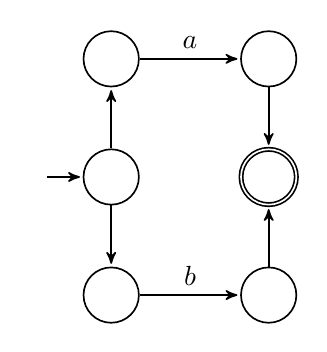
\begin{tikzpicture}[->, >=stealth', shorten >=1pt, auto, semithick, every state/.style={inner sep=0pt, minimum size=20pt}]
		\node[state, initial, initial text=]	(3) at (0, 0) {};
		\node[state]							(4) at (0, 1.5) {};
		\node[state]							(5) at (2, 1.5) {};
		\node[state]							(6) at (0, -1.5) {};
		\node[state]							(7) at (2, -1.5) {};
		\node[state, accepting]				(8) at (2, 0) {};
		
		\path 	(3) edge (4)
				(3) edge (6)
				(4) edge node{$a$} (5)
				(5) edge (8)
				(6) edge node{$b$} (7)
				(7) edge (8);
	\end{tikzpicture}
	\caption{NFA für \( (a + b) \)}
	\label{fig:re1}
\end{figure}
Um den Kleene'schen Abschluss zu bilden ergänzen wir einige (eigentlich überflüssige, aber nach Konstruktion erforderliche) Zustände. Man sieht wie der Automat aus Abbildung~\ref{fig:re1} eingebettet ist in den neuen Automaten in Abbildung~\ref{fig:re2}.\\
\begin{figure}[h]
	\centering
	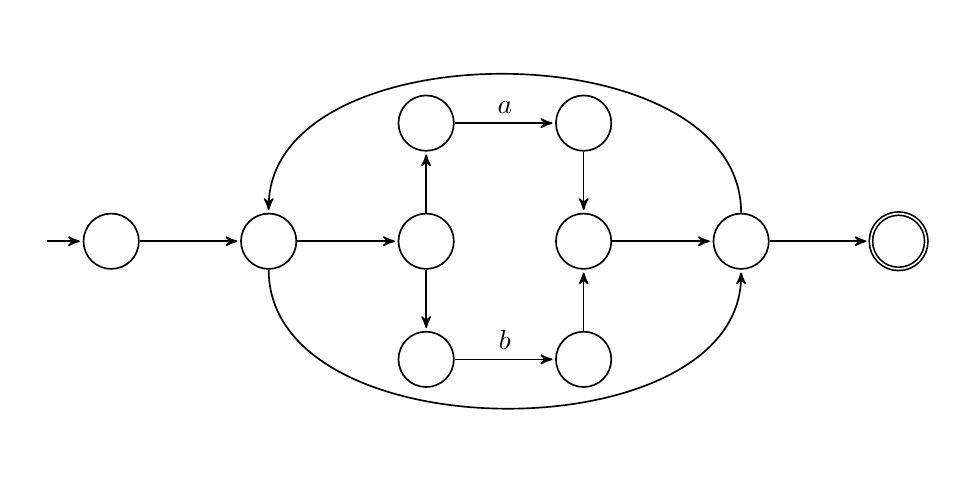
\begin{tikzpicture}[->, >=stealth', shorten >=1pt, auto, semithick, every state/.style={inner sep=0pt, minimum size=20pt}]
		\node[state, initial, initial text=]	(1) at (-4, 0) {};
		\node[state]							(2) at (-2, 0) {};
		\node[state]							(3) at (0, 0) {};
		\node[state]							(4) at (0, 1.5) {};
		\node[state]							(5) at (2, 1.5) {};
		\node[state]							(6) at (0, -1.5) {};
		\node[state]							(7) at (2, -1.5) {};
		\node[state]							(8) at (2, 0) {};
		\node[state]							(9) at (4, 0) {};
		\node[state, accepting]				(10) at (6, 0) {};
		
		\path 	(1) edge (2)
				(2) edge (3)
				(2) edge[bend right=90] (9)
				(3) edge (4)
				(3) edge (6)
				(4) edge node{$a$} (5)
				(5) edge (8)
				(6) edge node{$b$} (7)
				(7) edge (8)
				(8) edge (9)
				(9) edge (10)
				(9) edge[bend right=90] (2);
	\end{tikzpicture}
	\caption{NFA für \( (a + b)^\ast \)}
	\label{fig:re2}
\end{figure}
Zuletzt die Konkatenation von \( c \): Dazu fügen wir eine \(\varepsilon\)-Transition vom (noch) akzeptierenden Zustand vom Automaten in Abbildung~\ref{fig:re2} zum Startzustand des trivialen Automaten für die Sprache \( \{ c \} \). Der fertige Automat ist in Abbildung~\ref{fig:re3}.\\
\begin{figure}[h]
	\centering
	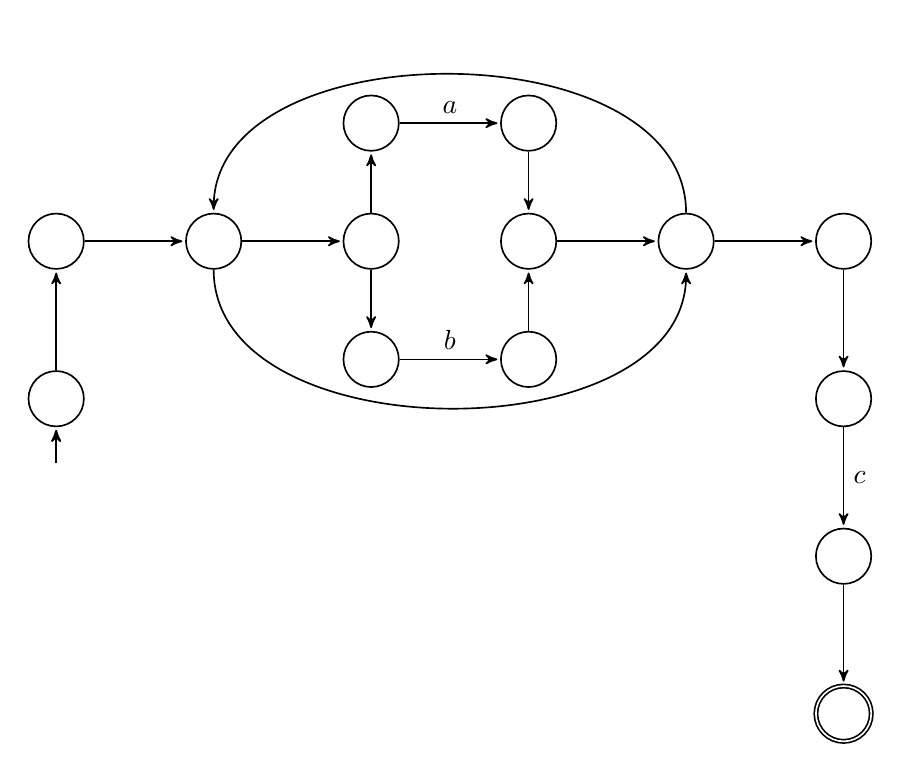
\begin{tikzpicture}[->, >=stealth', shorten >=1pt, auto, semithick, every state/.style={inner sep=0pt, minimum size=20pt}]
		\node[state, initial, initial text=, initial below]	(0) at (-4, -2) {};
		\node[state]											(1) at (-4, 0) {};
		\node[state]											(2) at (-2, 0) {};
		\node[state]											(3) at (0, 0) {};
		\node[state]											(4) at (0, 1.5) {};
		\node[state]											(5) at (2, 1.5) {};
		\node[state]											(6) at (0, -1.5) {};
		\node[state]											(7) at (2, -1.5) {};
		\node[state]											(8) at (2, 0) {};
		\node[state]											(9) at (4, 0) {};
		\node[state]											(10) at (6, 0) {};
		\node[state]											(11) at (6, -2) {};
		\node[state]											(12) at (6, -4) {};
		\node[state, accepting]								(13) at (6, -6) {};
		
		\path 	(0) edge (1)
				(1) edge (2)
				(2) edge (3)
				(2) edge[bend right=90] (9)
				(3) edge (4)
				(3) edge (6)
				(4) edge node{$a$} (5)
				(5) edge (8)
				(6) edge node{$b$} (7)
				(7) edge (8)
				(8) edge (9)
				(9) edge (10)
				(9) edge[bend right=90] (2)
				(10) edge (11)
				(11) edge node {$c$} (12)
				(12) edge (13);
	\end{tikzpicture}
	\caption{NFA für \( (a + b)^\ast c \)}
	\label{fig:re3}
\end{figure}
In den Hausaufgaben müsst ihr das nicht so ausführlich machen. Es reicht der Automat der Am Ende rauskommt. Ihr sollt aber das Verfahren aus der Vorlesung benutzen. Der Automat in Abbildung~\ref{fig:ref} ist zwar viel kleiner und äquivalent, aber nicht zulässig.
\begin{figure}[h]
	\centering
	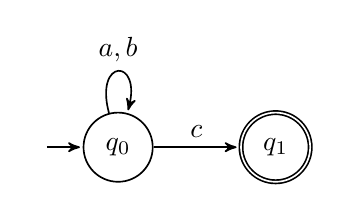
\begin{tikzpicture}[->, >=stealth', shorten >=1pt, auto, semithick]
		\node[state, initial, initial text=] (0) at (0, 0) {$q_0$};
		\node[state, accepting] (1) at (2, 0) {$q_1$};
		
		\path (0) edge[loop above] node {$a, b$} (0)
			(0) edge node {$c$} (1);
	\end{tikzpicture}
	\caption{Ein minimaler NFA für die Sprache \( L((a+b)^\ast c) \).}
	\label{fig:ref}
\end{figure}
\end{document}